\section{A quick start guide}\label{sec:quickstart}
  \subsection{xorb}\label{sec:quickstart:xorb}
  \subsection{xosoap}\label{sec:quickstart:xosoap}
  The aim of this quick start section is to provide you with all the
  critical information required to get you started with integrating SOAP
  in your OpenACS application in terms of consuming an existing SOAP
  service and providing your own as quick as possible. We provide
  ready-made and take-away code snippets and discuss the important steps
  in further detail. At some point, we might refer to further readings
  or more advanced concepts.
  \begin{hints}
  \item By referring to "SOAP" throughout the quick start section, we,
    more precisely, take into consideration SOAP 1.1
    \cite{w3c:2000}. Moreover, we exclusively refer to RPC as messaging or
    rather (de-)marshaling style. So, any occurrence of "SOAP" should
    actually be read as "SOAP-RPC 1.1".
  \end{hints}
  \subsubsection{How to glue to...?}\label{sec:xosoap:quickstart:glueto} 
  Say, you want to realise a scenario as depicted in Figure
\ref{fig:quickstart:xosoap:1}, i.e. you want to use the simple echo
functionality provided by a remote object or remote procedure through
SOAP. In this example scenario, we take a remote SOAP service called
EchoService as a given. It might realised either in xosoap itself or
any other SOAP infrastructure framework, such as gSOAP, Apache Axis,
.NET Remoting and the like. Further, we assume that EchoService
features a call "echoFloat" that requires a single argument of type
"float" (as defined as "built-in" simple type by the XML schema
specification) as input and promises to return a value of the very
same type. How do you call and consume this little example SOAP
service by means of xosoap?
\begin{hints}
\item As for data type declarations to be used on OpenACS Service
  Contracts or remoting protocols, there is a section in this manual
  dedicated to this issue (see Section \ref{sec:avanced:types}). For the
  scope of this quick start section, all (data) types refer to what is
  known as "built-in" primitive types as defined by XML schema
  specification 1.0 \cite{w3c:2004}. In xorb, there is a distinction
  between data types tags you can use in specifying contracts and the
  type handler behind the scenes. The former, e.g. xsFloat in the below
  example, are called \emph{type codes}, the actual handler (an XOTcl
  object) is an \emph{anything}.
\end{hints}
\begin{figure}[htbp]
  \begin{center}
    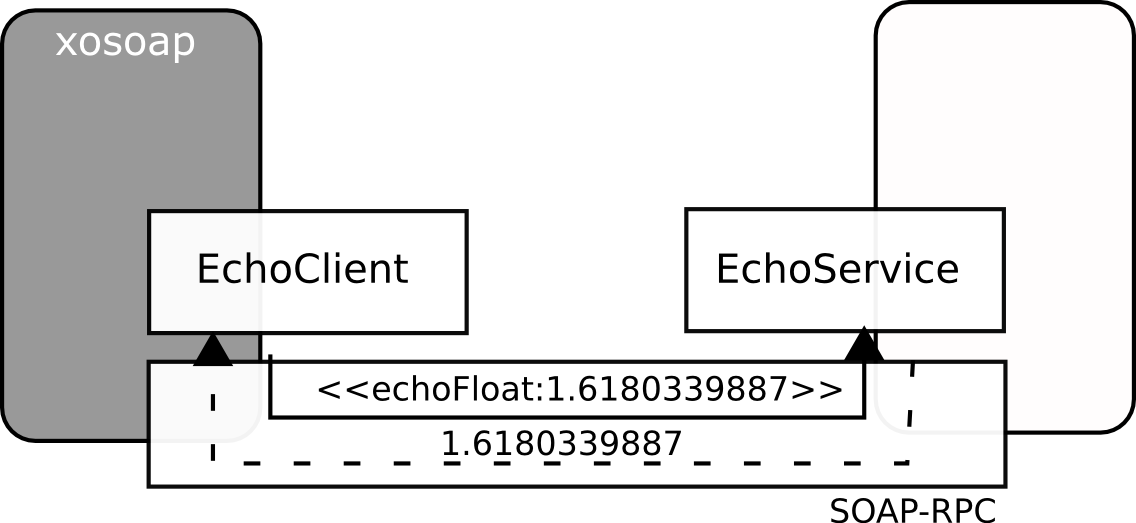
\includegraphics[scale=0.5]{img/consumer.png}
    \caption{Our example scenario}
    \label{fig:quickstart:xosoap:1}
  \end{center}
\end{figure}
\begin{hints}
\item Hold on! If you prefer to skip the little code walk below, just
  look at the underlying and deployable example scripts. You might want
  to go for a stand-alone sample script named
  ``example-01-soap-consumer.tcl'', located in
  xotcl-request-broker/www/doc/manual/examples/xosoap/. Alternatively,
  look in the corresponding test suite
  ``XosoapQuickStartEchoConsumer.suite'' residing at
  xotcl-request-broker/www/admin/storm. All line numbers provided
  along with the listings below refer to this test suite, for your convenience.
\item Interested in more details on a few flavours for realising soap
  clients: \ref{sec:advanced:interface:what}
\end{hints}
You just need four little steps and a few lines of code to get there:
\begin{enumerate}
\item Provide SOAP-specific configuration information as \emph{glue
    object}. To be concrete, create an instance of the XOTcl class
  \objlink{::xosoap::SoapGlueObject} and initiate the newly created
  object with some important bits of information:
  % firstline=6,lastline=10
  \lstset{breaklines=true,numbers=left,basicstyle=\footnotesize,frame=single,tabsize=3}
  % \lstinputlisting[firstnumber=1,name=example01,linerange={6-10}]{../examples/xosoap/example-01-soap-consumer.tcl}
  \lstinputlisting[firstnumber=auto,linerange=lst:quickstart:xosoap:1:step1-end,name=lst_quickstart_xosoap_1]{../../../admin/storm/XosoapQuickStartEchoConsumer.suite}

  In these few lines, we create and initiate an instance of the glue
  object class and provide three information bits to it. In the top line, we
  pass the actual endpoint address. In a conventional setting, the
  transport endpoint corresponds to a valid unique resource identifier
  (URL) as required by the HTTP protocol as transport provider. 
  % Line 4 also meets an information requirement at the HTTP level, i.e. the
  % value assigned to a specific HTTP header field prescribed by SOAP 1.1
  % \cite{w3c:2000} (and 1.2) specifications: the SOAPAction header
  % field. Line 2 and the setter call on callNamespace, on the contrary,
  % refers to a higher protocol level, i.e. the SOAP level. The value of
  % callNamespace will be used to set the namespace attached to the
  % method-describing element. This is used by a few SOAP frameworks,
  % e.g. .NET Remoting, to dispatch the remote call correctly to the
  % responsible servant. 
  For a detailed list of advanced configuration options, please, refer to
  \objlink{::xosoap::SoapGlueObject}.

  Want to learn more ...
  \begin{hints}
  \item ... about what 'glue objects' are? See
    \ref{sec:advanced:xorb:gobjects:what}
    % context object > principles of argument parsing
  \item ... about re-using 'glue object' to easen your tasks? See
    \ref{sec:advanced:xorb:gobjects:why}
    % concatenation of shadow information
  \end{hints}
  
\item Create a local proxy of the remote object or remote procedure, a
  so called \emph{client proxy}. This client proxy object holds a proxy
  method for the remote method or procedure to call. There are a few
  flavours for specifying such a client proxy, the most straight
  forward, however, is by instantiating
  \objlink{::xorb::stub::ProxyObject} and thus creating a proxy object.
  % \lstinputlisting[linerange={13-13},name=example01,firstnumber=last]{../examples/xosoap/example-01-soap-consumer.tcl}
  \lstinputlisting[firstnumber=auto,linerange=lst:quickstart:xosoap:1:step2-end,name=lst_quickstart_xosoap_1]{../../../admin/storm/XosoapQuickStartEchoConsumer.suite}
  
  The only significant step here is to associate the previously
  defined glue object to the client proxy. The information encapsulated
  by the glue object is then used by the underlying infrastructure to
  perform the actual remote call out of the combined information of the
  glue object and the client proxies interface. So, there it is, what we
  are still missing is the very client proxy.
\item Specify and realise the interface of your client proxy. The
  notion of object interfaces, to keep it simple, refers to the set
  methods and their method signatures defined on the object. When
  looking at Figure \ref{fig:quickstart:xosoap:1}, we learn that the
  interface of the remote object EchoService is quite simplistic: There
  is a single method echoFloat that takes a single argument flagged
  "inputFloat". The argument is, apart from a concrete label, further
  qualified by a type constraint called xsFloat. These type constraints
  are realised as
  \href{http://media.wu-wien.ac.at/doc/tutorial.html#non-pos-args}{check
    options on non-positional arguments}, in XOTcl terms. Besides, the
  interface promises a specific return value type, stipulated by passing
  a type code value as non-positional argument "returns" to ad\_proc.
  % \lstinputlisting[firstline=16,lastline=21,firstnumber=last]{../examples/xosoap/example-01-soap-consumer.tcl}
  \lstinputlisting[firstnumber=auto,linerange=lst:quickstart:xosoap:1:step3-end,name=lst_quickstart_xosoap_1]{../../../admin/storm/XosoapQuickStartEchoConsumer.suite}
  
  The method ad\_proc that comes with \objlink{::xorb::ProxyObject}
  overloads ad\_proc as defined on ::xotcl::Object, see
  \proclink{::xorb::ProxyObject}{instproc}{ad\_proc} a detailed
  description.
\item Invoke the proxy method to perform the remote call
%\lstinputlisting[firstline=23,lastline=23,firstnumber=last]{../examples/xosoap/example-01-soap-consumer.tcl}
  \lstinputlisting[firstnumber=auto,linerange=lst:quickstart:xosoap:1:step4-end,name=lst_quickstart_xosoap_1]{../../../admin/storm/XosoapQuickStartEchoConsumer.suite}
\end{enumerate}
So far, it needed three declarative steps to realise a call to a SOAP
service. The public interface of xosoap comes with various levels of
granularity (see \ref{sec:advanced:interface:what}) with the above
example referring to the medium-level interface. The higher-level one
allows to realise the previous example in a total of three steps with
only two declarative ones. Let's rewrite the example:

\begin{enumerate}
\item The major difference is that step 1 and 2 of the previous
  procedure are merged into one single step. Note, we now take advantage
  of a construct that natively comes with xosoap, the class
  \objlink{::xosoap::client::SoapObject}. This makes it completely
  sufficient, for instance, to import from the Tcl namespace
  ::xosoap::client::* without any need to use facilities of xorb
  directly (see full code snippet of the following example in Listing
  \ref{lst:quickstart:xosoap:3}.)
  \lstset{breaklines=true,numbers=left,basicstyle=\footnotesize,frame=single,tabsize=2}
  % \lstinputlisting[firstnumber=1,firstline=5,lastline=9]{../examples/xosoap/example-02-soap-consumer.tcl}
  \lstinputlisting[firstnumber=auto,linerange=lst:quickstart:xosoap:2:step1-end,name=lst_quickstart_xosoap_2]{../../../admin/storm/XosoapQuickStartEchoConsumer.suite}
\item The second step is, again, devoted to the declaration of the
  actual proxy interface, a local realisation of the echoFloat method on
  our combined proxy client and glue object:
%\lstinputlisting[firstnumber=last,firstline=12,lastline=18]{../examples/xosoap/example-02-soap-consumer.tcl}
  \lstinputlisting[firstnumber=auto,linerange=lst:quickstart:xosoap:2:step2-end,name=lst_quickstart_xosoap_2]{../../../admin/storm/XosoapQuickStartEchoConsumer.suite}
\item Finally, once the above is done, you can continue by issuing the
  call, i.e. invoke on the "remote" method:
  % \lstinputlisting[firstnumber=last,firstline=21,lastline=21]{../examples/xosoap/example-02-soap-consumer.tcl}
  \lstinputlisting[firstnumber=auto,linerange=lst:quickstart:xosoap:2:step3-end,name=lst_quickstart_xosoap_2]{../../../admin/storm/XosoapQuickStartEchoConsumer.suite}
\end{enumerate}

\begin{hints}
\item See the complete example: Listing
  \ref{lst:quickstart:xosoap:3}. All examples are dumped into the
  following directory, ready to pick them up:
  xotcl-soap/www/manual/examples. More recently, all examples are
  bundled as a test suite, ``XosoapQuickStartEchoConsumer.suite'' in
  xotcl-request-broker/www/admin/storm.
\item See (also for more example walk-throughs) Section
  \ref{sec:advanced:interface:what}
\end{hints}
  
  \subsubsection{Getting glued to ...?}
  In this section, we will briefly look at some straight-forward ways
  to expose your OpenACS code as a SOAP-based service. For this very
  purpose, we, again, consider the scenario as introduced in the
  previous section, but this time, we shift focus. Now, we want xosoap
  to realise the EchoService, the callee, and not, as previously, the
  EchoClient, i.e. the caller. Figure \ref{fig:quickstart:xosoap:2}
  indicates that we now aim at realising a service that offers a single
  remote method, i.e. "echoFloat", that takes a single argument of type
  "float" (again, as prescribed by the XML schema specfication) and is
  to echo the value of the argument back to the caller, again as XML
  schema built-in "float". The service laterally reverses the scenario
  in the previous section (see Section
  \ref{sec:xosoap:quickstart:glueto}). How can you achieve this?
  
  \begin{enumerate}
  \item Declare and deploy an \emph{interface description}. In
    OpenACS, interface descriptions have a long-standing tradition,
    however, sometimes neglected. You might be familiar with or, at least,
    you might have heart of \emph{service contracts} as provided by the
    OpenACS core. If not, don't panic! For the time being, you just need
    to know that there is something called "service contract" in OpenACS,
    that xorb builds upon this core feature of OpenACS and that you now
    need to create such a service contract, weird enough. Think of an
    interface description as a fundamental sketch of an object interface
    that lays down how the interface of a remote object and the interfaces
    of client proxies mimicking this remote object are to be construed. As
    for the EchoService in Figure \ref{fig:quickstart:xosoap:2}, a
    description might look the following way:
    \lstset{breaklines=true,numbers=left,basicstyle=\footnotesize,frame=single}
    \lstinputlisting[firstnumber=1,firstline=9,lastline=23]{../examples/xosoap/example-07-soap-provider-init.tcl}
    The above statement is, in the very literal sense of the word, a
    descriptive cast of a concrete EchoService service. Apart from a few
    bits of information targeting you as developer, it outlines that any
    servant or client proxy is meant to implement a method called
    "echoFloat", accepting a single argument and, in particular, throwing
    back a return value of a specific type. Don't forget to "deploy" your
    newly created service contract by calling:
    \lstinputlisting[firstnumber=last,firstline=26,lastline=26]{../examples/xosoap/example-07-soap-provider-init.tcl}
    This separate step of deployment might seem an overhead in this simple
    example, but it renders useful when considering more complex scenarios
    of designing and lifecycling interface descriptions.
    \begin{hints}
    \item There is a shrinking violet of an inline documentation available, see in particular, \objlink{::xorb::ServiceContract} and \objlink{::xorb::Abstract}.
    \end{hints}
  \item Provide servant code and register it with the invocation
    mechanism. The lines above are, as the notion of "interface
    description" implies, are mere description of something. What about
    the realisation of that something, i.e. the actual code block that is
    executed when the service is called. We refer to this code artefact as
    servant code or \emph{servant}, in short. But simply creating servant
    code is not enough, you still have to let xorb know which code block
    to invoke when calls from client proxies occur. The latter is referred
    to as providing a "service implementation", i.e. registering your code
    piece as realisation of a specific service contract! Behind the scenes
    and in some use cases, it might be more appropriate to deal with these
    two steps separately, however, in a straight-forward
    "get-me-a-soap-service" scenario, xorb provides a short cut to
    accomplish both in a single step:
    \lstinputlisting[firstnumber=last,firstline=30,lastline=38]{../examples/xosoap/example-07-soap-provider-init.tcl}
    The non-positional argument \emph{-implements} identifies the service
    contract realised by the underlying servant code, while \emph{-using}
    allows for specifying the intended delegations, which concrete code
    block is meant to be called for which abstract call. In our concrete
    example, we both provide a servant method called echoFloat and, behind
    the scenes, this servant method is registered as callee for abstract
    calls on echoFloat as defined by the contract. Note that the facility
    \objlink{::xorb::Method} is actually an XOTcl object (i.e. a slot
    object, to be more precise) that mimics the declaration of instprocs
    and procs as known from XOTcl. Finally, also deploy your service
    implementation:
    \lstinputlisting[firstnumber=last,firstline=41,lastline=41]{../examples/xosoap/example-07-soap-provider-init.tcl}
    At this point, you have accomplished most of the work needed to
    provide your EchoService. Two things remain to be done:
    \begin{hints}
    \item Interested in some background reading on OpenACS's service contracts? See the Section \ref{sec:internal:contracts}.
    \item See the complete Listing \ref{lst:quickstart:xosoap:7}.
    \item Again, you might also want to watch out the API Browser for information on \objlink{::xorb::ServiceImplementation}, \objlink{::xorb::Delegate}, and \objlink{::xorb::Method}.
    \end{hints}
  \item You might have asked yourself, while going through step 1 and
    2, where to actually put your the code outline above. Well, there are
    several answers to this question, you may choose between the following
    options:
    \begin{itemize}
    \item Your package's library files (*-procs.tcl, *-init.tcl):
      Preferably, drop your code in files situated in the tcl-subdirectory
      of your package. In either case, whether you choose a *-procs or a
      *-init file, make sure that you place the following line before the
      actual code block depicted in step 1 and 2:
      \lstinline[breaklines=true]!::xo::db::package require
      xotcl-request-broker!. Besides, there is a subtle difference between
      the *-procs and *-init files. The latter are evaluated only once,
      during server start-up. This means, contracts and implementations are
      only evaluate once. If you constantly develop, let's say, the servant
      code declared by your implementation, and you want your modifications/
      improvements to take effect without a dedicated server re-start, go
      for the *-procs option. This way, you can take advantage of xorb's
      reload and watch support.
    \item Your package's W(eb) U(user) I(nterface) files: In principle,
      you can specify a contract (::xorb::ServiceContract) in one of your
      www-subdirectory files as well. While it limits their usage, it does
      not break any functionality. Implementations
      (::xorb::ServiceImplementation) might as well be specified in WUI
      files, however, only the most basic variant makes sense in this
      context. The code of step 2 would not make sense as it defines servant
      code as well which should be available for all connections, i.e. in
      the context of all connection threads, and not only the one you
      specified it in by calling the WUI file.
    \item Developer shell: You can also drop the code in the shell as
      provided by the Developer Support package, however, the limitations
      for WUI scripts apply here as well.
    \end{itemize}
    
  \end{enumerate}
  \begin{figure}[htbp]
    \begin{center}
      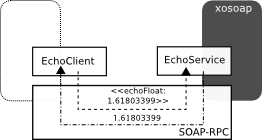
\includegraphics[width=0.5\textwidth]{img/provider.png}
      \caption{Our example scenario -- The provider side}
      \label{fig:quickstart:xosoap:2}
    \end{center}
  \end{figure}
  
  Finally, we want to look at two further nifty features for writing
  the callee interface, i.e. the service implementation, and
  servants. The first one refers to what is known as
  \objlink{::xorb::Delegate}, yet another way of linking abstract
  definitions to concrete servant code blocks. First, the above example
  could be rewritten in a probably common scenario. Just imagine, you
  previously created a piece of code (e.g., a proc) and you simply want
  to expose this artefact as servant instead of creating one by using
  \objlink{::xorb::Method} as shown above.  Or, you simply articulate
  the requirement that you keep prospective servant code and mere
  registration or binding code neatly seperated. In either case, you can
  revert to the use of little forwarding feature,
  i.e. \objlink{::xorb::Delegate}. Let's rewrite Listing
  \ref{lst:quickstart:xosoap:7} accordingly:
  
  The starting point is the assumption that there is an existing code
  block that we want taking the role of a servant for the abstract
  echoFloat method defined by our example contract. This particular proc
  might take the following form:
  \lstset{breaklines=true,numbers=left,basicstyle=\footnotesize,frame=single}
  \lstinputlisting[firstnumber=1,firstline=6,lastline=10]{../examples/xosoap/example-10-soap-provider-init.tcl}
  
  In view of our code base, we could then rewrite our service
implementation the following way, using \objlink{::xorb::Delegate}.
  
\lstinputlisting[firstnumber=last,firstline=39,lastline=47]{../examples/xosoap/example-10-soap-provider-init.tcl}

Let's, for a second, neglect some minor varations we introduced in the
above lines and that might distract. Key to the example is that the
service implementation now, once the specification has been
successfully processed, won't host any callable method on its own, it
rather acts as forwarder to your candidate proc. This delegation step
is realised by providing an absolute and qualified reference to the
target proc to the non-positional argument \lstinline!-for!. Apart
from the changed semantics, it will produce the same result as Listing
\ref{lst:quickstart:xosoap:7}. Some refinements are also shown in the
above snippet that did not show up in the introductory listing.  You
might have spotted that \objlink{::xorb::Delegate} takes a couple of
extra parameters. The same set is available for
\objlink{::xorb::Method}. In fact, both support all parameters known
from ad\_proc (or ad\_instproc). In addition, they come with an
optional parameter \lstinline!-per-object!. If you are familiar with
XOTcl, you will have noticed that methods, and beyond, can be declared
directly on objects or for instances of the declaring
object. Therefore, the distinction between "proc" and "instproc", just
to name the most prominent one. Similarily, you define the
\objlink{::xorb::Delegate} and \objlink{::xorb::Method} either at the
per-object or per-instance level. Behind the scenes, xorb's invocation
mechanism detects either way and will handle dispatches accordingly.
\begin{hints}
\item You might want to check out the API Browser for
  \objlink{::xorb::Delegate} and \objlink{::xorb::Method}.
\end{hints} 
As you just learnt, \objlink{::xorb::Delegate} provides
for rather simple delegating dispatch of abstract calls. A thorough
look at the above example of a serving proc, i.e. "servantProc", might
have created some suspicion: Tcl procs allow for positional argument
passing, if we neglect the ad\_proc facility of OpenACS for a
second. However, xorb is primarily built around non-positional
arguments. We briefly mentioned this fact while describing the
semantics of \objlink{::xorb::Abstract}. This is due to the fact that
xorb heavily uses
\href{http://media.wu-wien.ac.at/doc/tutorial.html#non-pos-args}{XOTcl
  check options} that are (at least up to the 1.5.x generation)
exclusively available to non-positional arguments. Besides, most
remoting protocols, including SOAP and XML-RPC adopted this pattern of
argument passing \cite{zdun:2005b}.

Be that as it may, it leaves xorb with servants that do not take
non-positional arguments. However, thanks to (XO)Tcl's introspective
capabilities, xorb provides for \emph{argument bridging}. It will
identify the type of servant code block and adapt the pending call
dispatch accordingly, including the rewrite of the passed
argument-value list. Note, there are of course limitations to this
approach, namely if you consider mixed signatures, containing both
positional and non-positional arguments.

%%% Local Variables: 
%%% mode: latex
%%% TeX-master: "../../../../../../../win/workspace/dev/xotcl-request-broker/www/doc/manual/src/manual"
%%% End: 
